% ---------------------------------------------------------------------------------------------
%
% https://github.com/dTmC0945/C-MCI-LaTeX-Class-mcidoc
%
% ---------------------------------------------------------------------------------------------

\documentclass[   
state        = Report,                       % (Report | Slide    | Thesis)
lang         = DE,                           % (DE     | EN) 
degree       = BSc,                          % (BSc    | MSc)
dept         = MECH,                         % (MECH   | SBT)
bib-active   = true,                         % (true   | false)
bib-style    = ieee,                         % (ieee)
column-type  = one,                          % (one    | two)
]{mcidoc}

% CUSTOM COMMANDS -----------------------------------------------------------------------------
%       
% Please enter any custom command/packages you require here for easy tracking 

\usepackage{float}
\usepackage{siunitx}
\usepackage{svg}

\sisetup{
	locale = DE,            % Deutsche Einstellungen, z. B. Dezimalkomma
	per-mode = symbol,      % Einheiten wie „m/s“ statt m s⁻¹
}

% For example, bibliography setting are added. Bibtex is the standard but if you prefer
% there are other options on the market such as biber. Style has been chosen as IEEE but if 
% are from another discipline, please feel free to change it.

%\bibliography{references.bib}  % Here we add our file where we store our references.
%      
% ---------------------------------------------------------------------------------------------

% DOCUMENT PARAMETERS -------------------------------------------------------------------------

\TitleHeader{ $ $ }

\Title{%
  Laborbericht
}% 

\Lecture{Elektrotechnik I}%    

\Lecturer{Dr. Georg Saxl}%

\Cohort{BA-MECH-25}%           
\Group{BA-MECH-25-2A}%

\StudentName{Stefan Höllrigl, Noah Kandziora, Vsevolod Kopus}%
\StudentID{2510602025, 2510602059, 2410602042}% 

%\Supervisor{Colin Stevens}%

\begin{document} % ############################################################################

\MakeTitlePage     

\TableOfContents           

% REPORT CONTENT ------------------------------------------------------------------------------

% ----      
% Your report content should go here and should follow structure befitting of a scientific
% report and should be written in a scientific format. For more information please look at
% MCI guidelines on how it should be done.      
% ----  


\include{chapter/introduction.tex}   % nur zur Demonstration
%---------------------------------------------------------------------
\setcounter{chapter}{1}
\chapter{Gleichstromtechnik}
%---------------------------------------------------------------------
\setcounter{section}{1}
\setcounter{subsection}{1}

\subsection{Ohmsches Gesetz}

Die Erdbeschleunigung beträgt \SI{9.81}{\meter\per\second\squared}.\\
Wie in Abbildung~\ref{fig:meinplot} gezeigt, ...

\begin{figure}[H]
	\centering
	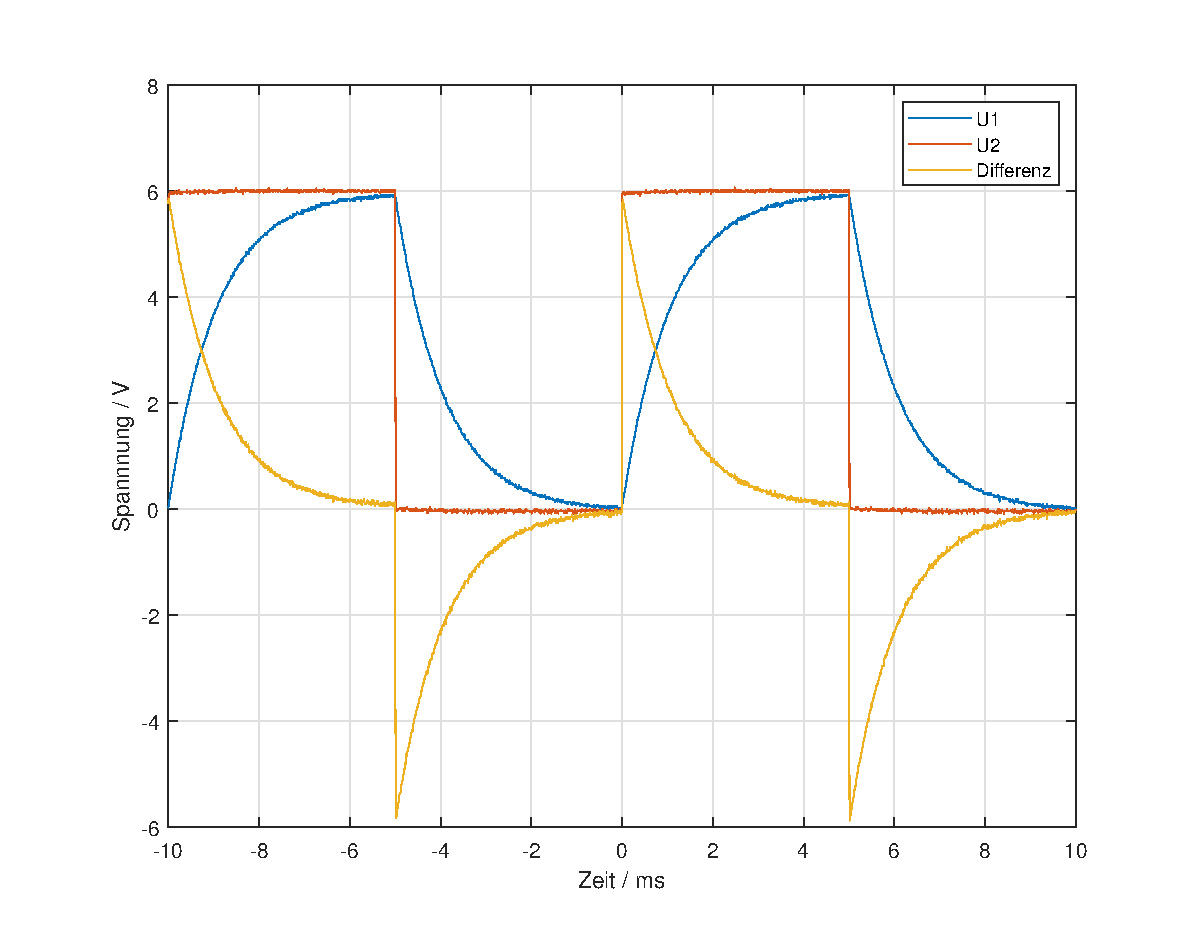
\includegraphics[width=0.8\textwidth]{img/Plot.eps}
	\caption{Meine Bildbeschreibung}
	\label{fig:meinplot}
\end{figure}


\subsubsection{Ergebnisse}

\subsubsection{Diskussion}


%---------------------------------------------------------------------
\newpage
\setcounter{section}{2}
\setcounter{subsection}{1}
\subsection{Mischen von Reihen- und Parallelschaltungen}

\subsubsection{Ergebnisse}

\subsubsection{Diskussion}


%---------------------------------------------------------------------
\newpage
\setcounter{section}{3}
\setcounter{subsection}{1}
\subsection{Unbelasteter Spannungsteiler}

\subsubsection{Ergebnisse}

\subsubsection{Diskussion}



%---------------------------------------------------------------------
\newpage
\setcounter{section}{4}
\setcounter{subsection}{1}
\subsection{Belasteter Spannungsteiler}

\subsubsection{Ergebnisse}

\subsubsection{Diskussion}



%---------------------------------------------------------------------
\newpage
\setcounter{section}{5}
\setcounter{subsection}{1}
\subsection{Spannungsrichtige und stromrichtige Messung}

\subsubsection{Ergebnisse}

\subsubsection{Diskussion}


%---------------------------------------------------------------------
\newpage
\setcounter{section}{6}
\setcounter{subsection}{1}
\subsection{Ersatzspannungsquelle}

\subsubsection{Ergebnisse}

\subsubsection{Diskussion}



%---------------------------------------------------------------------
\newpage
\setcounter{section}{7}
\setcounter{subsection}{1}
\subsection{Reihenschaltung von Spannungsquellen}

\subsubsection{Ergebnisse}

\subsubsection{Diskussion}


%---------------------------------------------------------------------
\newpage
\setcounter{section}{8}
\setcounter{subsection}{1}
\subsection{Parallelschaltung von Spannungsquellen}

\subsubsection{Ergebnisse}

\subsubsection{Diskussion}






   
%---------------------------------------------------------------------
\chapter{Kondensator im Wechselstromkreis}
%---------------------------------------------------------------------
\setcounter{section}{2}
\setcounter{subsection}{1}

\subsection{Lade- und Entladevorgang eines Kondensators}

\subsubsection{Ergebnisse}

\subsubsection{Diskussion}



%---------------------------------------------------------------------
\setcounter{section}{3}
\setcounter{subsection}{1}

\subsection{Phasenverschiebung zwischen Strom und Spannung am Kondensator}

\subsubsection{Ergebnisse}

\subsubsection{Diskussion}



%---------------------------------------------------------------------
\setcounter{section}{4}
\setcounter{subsection}{1}

\subsection{Kapazitiver Blindwiderstand eines Kondensators}

\subsubsection{Ergebnisse}

\subsubsection{Diskussion}



%---------------------------------------------------------------------
\setcounter{section}{7}
\setcounter{subsection}{1}

\subsection{Blindleistung eines Kondensators}

\subsubsection{Ergebnisse}

\subsubsection{Diskussion}



  
%---------------------------------------------------------------------
\chapter{Spule im Wechselstromkreis}
%---------------------------------------------------------------------
\setcounter{section}{2}
\setcounter{subsection}{1}

\subsection{Ein- und Ausschaltvorgang an einer Spule}

\subsubsection{Ergebnisse}

\subsubsection{Diskussion}



%---------------------------------------------------------------------
\setcounter{section}{3}
\setcounter{subsection}{1}

\subsection{Phasenverschiebung zwischen Strom und Spannung an einer Spule}

\subsubsection{Ergebnisse}

\subsubsection{Diskussion}





   
%---------------------------------------------------------------------
\chapter{Zusammenschaltung von Widerstand, Kondensator, Spule}
%---------------------------------------------------------------------
\setcounter{section}{5}
\setcounter{subsection}{1}

\subsection{Parallelschaltung von Widerstand und Spule}

\subsubsection{Ergebnisse}

\subsubsection{Diskussion}


%---------------------------------------------------------------------
\setcounter{section}{2}
\setcounter{subsection}{1}

\subsection{Reihenschaltung von Widerstand und Kondensator}

\subsubsection{Ergebnisse}

\subsubsection{Diskussion}


%---------------------------------------------------------------------
\setcounter{section}{10}
\setcounter{subsection}{1}

\subsection{Wirk-, Blind- und Scheinleistung}

\subsubsection{Ergebnisse}

\subsubsection{Diskussion}






   


% ---- 
% Add as many chapters as you see fit for your content. For easy legibility and for dynamic
% adjustment of content it would be suggested to write your files and place them similar to
% the aforementioned examples.

% REPORT POSTAMBLE ----------------------------------------------------------------------------

% ----
% In this section, please put all the thing you deem are necessary for the thesis but does have
% no substance as materials (i.e., technical drawings, patents, massive code bases).
% ----

%\printbibliography

% \makeindex
% \printnomenclature
% \printglossaries

\end{document} % ##############################################################################
